\chapter{Traceability and Change Management}

\begin{lernziele}
After this chapter, you can build end-to-end traceability from requirements to tests. You understand traceability chains, impact analysis, and the value of systematic change assessment in the robot project.
\end{lernziele}

\section{Introduction}
\gls{traceability} means you can trace how artifacts connect. In MBSE, this is one of the biggest practical benefits: requirements, functions, system parts, interfaces, ROS2 nodes, and tests stay connected.

\section{What Is Traceability?}
Traceability answers questions such as:

\begin{itemize}
    \item Which component satisfies this requirement?
    \item Which test verifies this requirement?
    \item Which ROS2 node implements this system element?
    \item Which interfaces are affected if a sensor changes?
    \item Which requirements still have no test?
\end{itemize}

\Needspace{12\baselineskip}
\section{A Chain in the Robot Project}
\begin{lstlisting}[style=plaintext]
REQ-002 Detect obstacles
-> PerceptionSystem
-> ObstacleDetector
-> obstacle_detector_node
-> /scan
-> TC-002 Obstacle detection
\end{lstlisting}

This chain shows how you can trace a requirement all the way to its implementation and test. In SysML v2, you can anchor such links directly in the model using the \texttt{satisfy}, \texttt{derive}, and \texttt{trace} relationships, for example:

\begin{lstlisting}
satisfy requirement REQ_002 by PerceptionSystem;
derive requirement REQ_002 from REQ_SAFE_002;
trace PerceptionSystem to obstacle_detector_node;
\end{lstlisting}

Figure~\ref{fig:kap20-traceability-kette-req002} shows the same chain graphically, including the type of relationship between each pair of elements.

\begin{figure}[H]
  \centering
  \adjustbox{max width=\linewidth,max totalheight=0.6\textheight}{% =====================================================================
% Figure: Traceability chain for REQ-002
% Matches Chapter 20, section "A Chain in the Robot Project"
%
% Used in the book, e.g. in chapters_en/20_traceability.tex:
%
%   \begin{figure}[H]
%     \centering
%     % =====================================================================
% Figure: Traceability chain for REQ-002
% Matches Chapter 20, section "A Chain in the Robot Project"
%
% Used in the book, e.g. in chapters_en/20_traceability.tex:
%
%   \begin{figure}[H]
%     \centering
%     % =====================================================================
% Figure: Traceability chain for REQ-002
% Matches Chapter 20, section "A Chain in the Robot Project"
%
% Used in the book, e.g. in chapters_en/20_traceability.tex:
%
%   \begin{figure}[H]
%     \centering
%     \input{figures_en/fig_kap20_traceability_kette_req002}
%     \caption{Traceability chain from REQ-002, through SysML system
%       elements and a ROS2 node/topic, to test case TC-002.}
%     \label{fig:kap20-traceability-kette-req002}
%   \end{figure}
%
% Required packages (already loaded in main_en.tex): tikz
% Required TikZ libraries: positioning, arrows.meta, shadows, calc
% =====================================================================

\input{figures_en/fig_kap20_traceability_kette_req002.tikz}

%     \caption{Traceability chain from REQ-002, through SysML system
%       elements and a ROS2 node/topic, to test case TC-002.}
%     \label{fig:kap20-traceability-kette-req002}
%   \end{figure}
%
% Required packages (already loaded in main_en.tex): tikz
% Required TikZ libraries: positioning, arrows.meta, shadows, calc
% =====================================================================

\begin{tikzpicture}[
    scale=0.85, transform shape,
    every node/.style={font=\small},
    req/.style={
        rectangle, rounded corners=1.5pt, draw=black!70, thick,
        minimum width=30mm, minimum height=11mm,
        align=center, fill=blue!12, drop shadow
    },
    part/.style={
        rectangle, rounded corners=1.5pt, draw=green!40!black, thick,
        minimum width=30mm, minimum height=11mm,
        align=center, fill=green!15, drop shadow
    },
    code/.style={
        rectangle, rounded corners=1.5pt, draw=orange!60!black, thick,
        minimum width=30mm, minimum height=11mm,
        align=center, fill=orange!15, drop shadow
    },
    test/.style={
        rectangle, rounded corners=1.5pt, draw=black!50, thick,
        minimum width=30mm, minimum height=11mm,
        align=center, fill=black!6, drop shadow
    },
    flow/.style={-{Stealth[length=2.2mm]}, thick, black!60},
    lbl/.style={font=\small, fill=white, inner sep=1pt}
]

% --- row 1: REQ -> system elements ---
\node[req]  (req002) at (0, 3)  {\texttt{REQ-002}\\Detect\\Obstacles};
\node[part] (percept) at (5, 3) {\texttt{Perception-}\\\texttt{System}};
\node[part] (detect)  at (10, 3) {\texttt{Obstacle-}\\\texttt{Detector}};

% --- row 2: implementation -> test (continuation of the chain) ---
\node[code] (node)  at (0, 0) {\texttt{obstacle\_}\\\texttt{detector\_node}};
\node[code] (topic) at (5, 0) {\texttt{/scan}};
\node[test] (tc002) at (10, 0) {\texttt{TC-002}\\Obstacle Detection};

% --- chain row 1 ---
\draw[flow] (req002)  -- node[lbl, midway]{\texttt{satisfy}}  (percept);
\draw[flow] (percept) -- node[lbl, midway]{\texttt{allocate}} (detect);

% --- transition row 1 -> row 2 ---
\draw[flow] (detect.south) -- node[lbl, midway]{\texttt{realize}} (node.north);

% --- chain row 2 ---
\draw[flow] (node)  -- node[lbl, midway]{publishes} (topic);
\draw[flow] (topic) -- node[lbl, midway]{\texttt{verify}} (tc002);

% --- legend ---
\node[req,  minimum width=6mm, minimum height=4mm, below=14mm of node, xshift=-6mm, font=\small] (leg1) {};
\node[right=1mm of leg1, font=\small, align=left] (lab1){Requirement};
\node[part, minimum width=6mm, minimum height=4mm, right=6mm of lab1, font=\small] (leg2) {};
\node[right=1mm of leg2, font=\small, align=left] (lab2){SysML system element};
\node[code, minimum width=6mm, minimum height=4mm, right=6mm of lab2, font=\small] (leg3) {};
\node[right=1mm of leg3, font=\small, align=left] (lab3){ROS2 node/topic};
\node[test, minimum width=6mm, minimum height=4mm, right=6mm of lab3, font=\small] (leg4) {};
\node[right=1mm of leg4, font=\small, align=left] (lab4){Test case};

\end{tikzpicture}


%     \caption{Traceability chain from REQ-002, through SysML system
%       elements and a ROS2 node/topic, to test case TC-002.}
%     \label{fig:kap20-traceability-kette-req002}
%   \end{figure}
%
% Required packages (already loaded in main_en.tex): tikz
% Required TikZ libraries: positioning, arrows.meta, shadows, calc
% =====================================================================

\begin{tikzpicture}[
    scale=0.85, transform shape,
    every node/.style={font=\small},
    req/.style={
        rectangle, rounded corners=1.5pt, draw=black!70, thick,
        minimum width=30mm, minimum height=11mm,
        align=center, fill=blue!12, drop shadow
    },
    part/.style={
        rectangle, rounded corners=1.5pt, draw=green!40!black, thick,
        minimum width=30mm, minimum height=11mm,
        align=center, fill=green!15, drop shadow
    },
    code/.style={
        rectangle, rounded corners=1.5pt, draw=orange!60!black, thick,
        minimum width=30mm, minimum height=11mm,
        align=center, fill=orange!15, drop shadow
    },
    test/.style={
        rectangle, rounded corners=1.5pt, draw=black!50, thick,
        minimum width=30mm, minimum height=11mm,
        align=center, fill=black!6, drop shadow
    },
    flow/.style={-{Stealth[length=2.2mm]}, thick, black!60},
    lbl/.style={font=\small, fill=white, inner sep=1pt}
]

% --- row 1: REQ -> system elements ---
\node[req]  (req002) at (0, 3)  {\texttt{REQ-002}\\Detect\\Obstacles};
\node[part] (percept) at (5, 3) {\texttt{Perception-}\\\texttt{System}};
\node[part] (detect)  at (10, 3) {\texttt{Obstacle-}\\\texttt{Detector}};

% --- row 2: implementation -> test (continuation of the chain) ---
\node[code] (node)  at (0, 0) {\texttt{obstacle\_}\\\texttt{detector\_node}};
\node[code] (topic) at (5, 0) {\texttt{/scan}};
\node[test] (tc002) at (10, 0) {\texttt{TC-002}\\Obstacle Detection};

% --- chain row 1 ---
\draw[flow] (req002)  -- node[lbl, midway]{\texttt{satisfy}}  (percept);
\draw[flow] (percept) -- node[lbl, midway]{\texttt{allocate}} (detect);

% --- transition row 1 -> row 2 ---
\draw[flow] (detect.south) -- node[lbl, midway]{\texttt{realize}} (node.north);

% --- chain row 2 ---
\draw[flow] (node)  -- node[lbl, midway]{publishes} (topic);
\draw[flow] (topic) -- node[lbl, midway]{\texttt{verify}} (tc002);

% --- legend ---
\node[req,  minimum width=6mm, minimum height=4mm, below=14mm of node, xshift=-6mm, font=\small] (leg1) {};
\node[right=1mm of leg1, font=\small, align=left] (lab1){Requirement};
\node[part, minimum width=6mm, minimum height=4mm, right=6mm of lab1, font=\small] (leg2) {};
\node[right=1mm of leg2, font=\small, align=left] (lab2){SysML system element};
\node[code, minimum width=6mm, minimum height=4mm, right=6mm of lab2, font=\small] (leg3) {};
\node[right=1mm of leg3, font=\small, align=left] (lab3){ROS2 node/topic};
\node[test, minimum width=6mm, minimum height=4mm, right=6mm of lab3, font=\small] (leg4) {};
\node[right=1mm of leg4, font=\small, align=left] (lab4){Test case};

\end{tikzpicture}

}
  \caption{Traceability chain from REQ-002, through SysML system elements and a ROS2 node/topic, to test case TC-002.}
  \label{fig:kap20-traceability-kette-req002}
\end{figure}

\section{Benefit}
If REQ-002 changes, you can analyze which components are affected. Maybe the lidar needs to be replaced. Maybe the test needs to be adjusted. Maybe a software change is enough.

\section{Impact Analysis}
Impact analysis answers the question: What changes if a requirement, component, or interface changes?

You can answer this question methodically by starting at the changed requirement and following the traceability matrix backward: which system elements, interfaces, ROS2 nodes, and tests are linked to it through a relationship?

Example: the maximum speed is increased. This can affect:

\begin{itemize}
    \item safety requirements
    \item the braking-distance model
    \item obstacle detection
    \item motor control
    \item battery runtime
    \item tests for stopping distance
    \item the ROS2 parameter for speed
\end{itemize}

\section{Traceability Matrix}
A simple matrix can have these columns:

\begin{itemize}
    \item requirement
    \item function
    \item SysML system element (\texttt{part def})
    \item ROS2 node
    \item interface
    \item test case
\end{itemize}

This matrix does not replace the model, but it is a useful view. Figure~\ref{fig:kap20-traceability-matrix} shows an excerpt for two requirements of the indoor robot. Modern SysML v2 tools can often generate such a matrix automatically from the model's relationships, which greatly reduces the effort of maintaining it by hand.

\begin{figure}[H]
  \centering
  \adjustbox{max width=\linewidth,max totalheight=0.6\textheight}{% =====================================================================
% Figure: Traceability matrix for the indoor robot (excerpt)
% Matches Chapter 20, section "Traceability Matrix"
%
% Used in the book, e.g. in chapters_en/20_traceability.tex:
%
%   \begin{figure}[H]
%     \centering
%     % =====================================================================
% Figure: Traceability matrix for the indoor robot (excerpt)
% Matches Chapter 20, section "Traceability Matrix"
%
% Used in the book, e.g. in chapters_en/20_traceability.tex:
%
%   \begin{figure}[H]
%     \centering
%     % =====================================================================
% Figure: Traceability matrix for the indoor robot (excerpt)
% Matches Chapter 20, section "Traceability Matrix"
%
% Used in the book, e.g. in chapters_en/20_traceability.tex:
%
%   \begin{figure}[H]
%     \centering
%     \input{figures_en/fig_kap20_traceability_matrix}
%     \caption{Excerpt from a traceability matrix: each row connects
%       a requirement, through a function, system element, and ROS2
%       node, to a test case.}
%     \label{fig:kap20-traceability-matrix}
%   \end{figure}
%
% Required packages (already loaded in main_en.tex): tikz
% Required TikZ libraries: positioning, arrows.meta, shadows, calc
% =====================================================================

\input{figures_en/fig_kap20_traceability_matrix.tikz}

%     \caption{Excerpt from a traceability matrix: each row connects
%       a requirement, through a function, system element, and ROS2
%       node, to a test case.}
%     \label{fig:kap20-traceability-matrix}
%   \end{figure}
%
% Required packages (already loaded in main_en.tex): tikz
% Required TikZ libraries: positioning, arrows.meta, shadows, calc
% =====================================================================

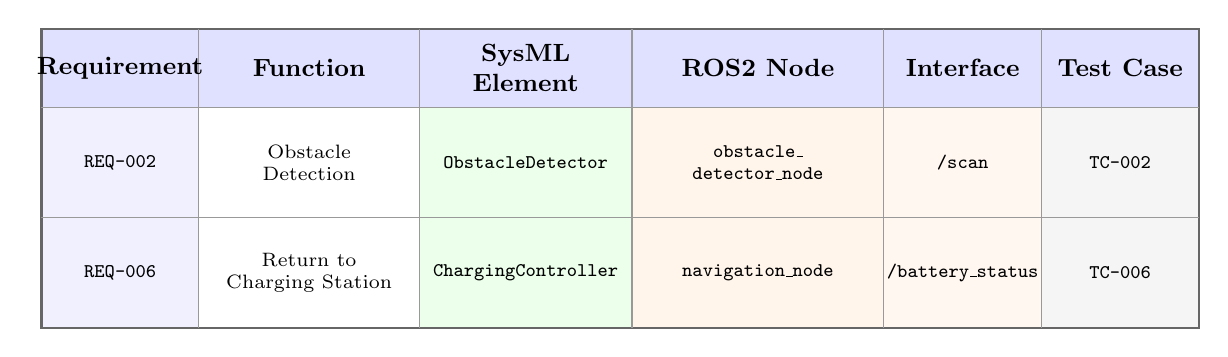
\begin{tikzpicture}[
    every node/.style={font=\small},
    x=1cm, y=1cm
]

% --- column boundaries (x) and row boundaries (y) in cm ---
% Columns: Requirement | Function | SysML system element | ROS2 node | Interface | Test case
% x0=0, x1=2.0, x2=4.8, x3=7.5, x4=10.7, x5=12.7, x6=14.7
% Rows (from top): y0=3.8 (header top), y1=2.8 (header bottom / row 1 top),
%                   y2=1.4 (row 1 bottom / row 2 top), y3=0 (row 2 bottom)

% --- column background for data rows (y3 to y1) ---
\fill[blue!6]   (0,0)    rectangle (2.0,2.8);
\fill[white]    (2.0,0)  rectangle (4.8,2.8);
\fill[green!8]  (4.8,0)  rectangle (7.5,2.8);
\fill[orange!8] (7.5,0)  rectangle (10.7,2.8);
\fill[orange!6] (10.7,0) rectangle (12.7,2.8);
\fill[black!4]  (12.7,0) rectangle (14.7,2.8);

% --- shade the header row on top ---
\fill[blue!12] (0,2.8) rectangle (14.7,3.8);

% --- grid lines: outer frame ---
\draw[black!60, thick] (0,0) rectangle (14.7,3.8);

% --- grid lines: vertical column separators ---
\draw[black!40] (2.0,0)  -- (2.0,3.8);
\draw[black!40] (4.8,0)  -- (4.8,3.8);
\draw[black!40] (7.5,0)  -- (7.5,3.8);
\draw[black!40] (10.7,0) -- (10.7,3.8);
\draw[black!40] (12.7,0) -- (12.7,3.8);

% --- grid lines: horizontal row separators ---
\draw[black!40] (0,1.4) -- (14.7,1.4);
\draw[black!40] (0,2.8) -- (14.7,2.8);

% --- header text ---
\node[font=\small\bfseries] at (1.0,3.3)  {Requirement};
\node[font=\small\bfseries] at (3.4,3.3)  {Function};
\node[font=\small\bfseries, align=center] at (6.15,3.3) {SysML\\Element};
\node[font=\small\bfseries] at (9.1,3.3)  {ROS2 Node};
\node[font=\small\bfseries] at (11.7,3.3) {Interface};
\node[font=\small\bfseries] at (13.7,3.3) {Test Case};

% --- row 1: REQ-002 ---
\node[font=\scriptsize] at (1.0,2.1)  {\texttt{REQ-002}};
\node[font=\scriptsize, align=center] at (3.4,2.1)  {Obstacle\\Detection};
\node[font=\scriptsize] at (6.15,2.1) {\texttt{ObstacleDetector}};
\node[font=\scriptsize, align=center] at (9.1,2.1)  {\texttt{obstacle\_}\\\texttt{detector\_node}};
\node[font=\scriptsize] at (11.7,2.1) {\texttt{/scan}};
\node[font=\scriptsize] at (13.7,2.1) {\texttt{TC-002}};

% --- row 2: REQ-006 ---
\node[font=\scriptsize] at (1.0,0.7)  {\texttt{REQ-006}};
\node[font=\scriptsize, align=center] at (3.4,0.7)  {Return to\\Charging Station};
\node[font=\scriptsize] at (6.15,0.7) {\texttt{ChargingController}};
\node[font=\scriptsize] at (9.1,0.7)  {\texttt{navigation\_node}};
\node[font=\scriptsize] at (11.7,0.7) {\texttt{/battery\_status}};
\node[font=\scriptsize] at (13.7,0.7) {\texttt{TC-006}};

\end{tikzpicture}


%     \caption{Excerpt from a traceability matrix: each row connects
%       a requirement, through a function, system element, and ROS2
%       node, to a test case.}
%     \label{fig:kap20-traceability-matrix}
%   \end{figure}
%
% Required packages (already loaded in main_en.tex): tikz
% Required TikZ libraries: positioning, arrows.meta, shadows, calc
% =====================================================================

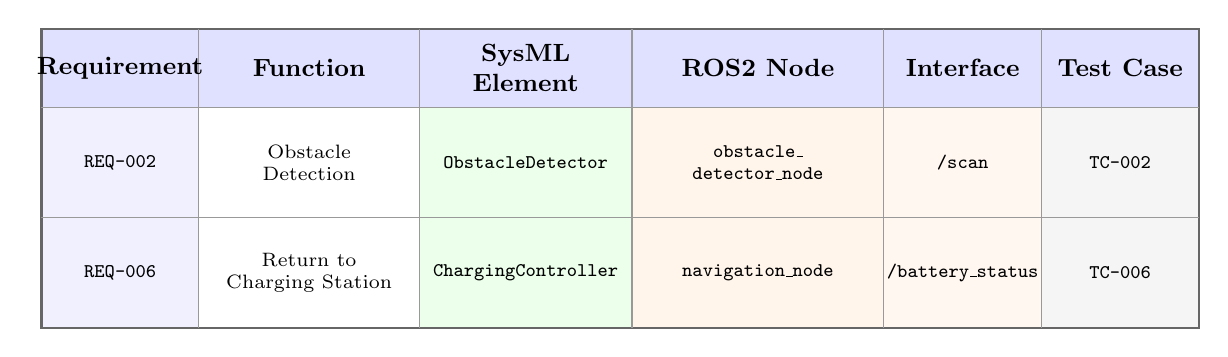
\begin{tikzpicture}[
    every node/.style={font=\small},
    x=1cm, y=1cm
]

% --- column boundaries (x) and row boundaries (y) in cm ---
% Columns: Requirement | Function | SysML system element | ROS2 node | Interface | Test case
% x0=0, x1=2.0, x2=4.8, x3=7.5, x4=10.7, x5=12.7, x6=14.7
% Rows (from top): y0=3.8 (header top), y1=2.8 (header bottom / row 1 top),
%                   y2=1.4 (row 1 bottom / row 2 top), y3=0 (row 2 bottom)

% --- column background for data rows (y3 to y1) ---
\fill[blue!6]   (0,0)    rectangle (2.0,2.8);
\fill[white]    (2.0,0)  rectangle (4.8,2.8);
\fill[green!8]  (4.8,0)  rectangle (7.5,2.8);
\fill[orange!8] (7.5,0)  rectangle (10.7,2.8);
\fill[orange!6] (10.7,0) rectangle (12.7,2.8);
\fill[black!4]  (12.7,0) rectangle (14.7,2.8);

% --- shade the header row on top ---
\fill[blue!12] (0,2.8) rectangle (14.7,3.8);

% --- grid lines: outer frame ---
\draw[black!60, thick] (0,0) rectangle (14.7,3.8);

% --- grid lines: vertical column separators ---
\draw[black!40] (2.0,0)  -- (2.0,3.8);
\draw[black!40] (4.8,0)  -- (4.8,3.8);
\draw[black!40] (7.5,0)  -- (7.5,3.8);
\draw[black!40] (10.7,0) -- (10.7,3.8);
\draw[black!40] (12.7,0) -- (12.7,3.8);

% --- grid lines: horizontal row separators ---
\draw[black!40] (0,1.4) -- (14.7,1.4);
\draw[black!40] (0,2.8) -- (14.7,2.8);

% --- header text ---
\node[font=\small\bfseries] at (1.0,3.3)  {Requirement};
\node[font=\small\bfseries] at (3.4,3.3)  {Function};
\node[font=\small\bfseries, align=center] at (6.15,3.3) {SysML\\Element};
\node[font=\small\bfseries] at (9.1,3.3)  {ROS2 Node};
\node[font=\small\bfseries] at (11.7,3.3) {Interface};
\node[font=\small\bfseries] at (13.7,3.3) {Test Case};

% --- row 1: REQ-002 ---
\node[font=\scriptsize] at (1.0,2.1)  {\texttt{REQ-002}};
\node[font=\scriptsize, align=center] at (3.4,2.1)  {Obstacle\\Detection};
\node[font=\scriptsize] at (6.15,2.1) {\texttt{ObstacleDetector}};
\node[font=\scriptsize, align=center] at (9.1,2.1)  {\texttt{obstacle\_}\\\texttt{detector\_node}};
\node[font=\scriptsize] at (11.7,2.1) {\texttt{/scan}};
\node[font=\scriptsize] at (13.7,2.1) {\texttt{TC-002}};

% --- row 2: REQ-006 ---
\node[font=\scriptsize] at (1.0,0.7)  {\texttt{REQ-006}};
\node[font=\scriptsize, align=center] at (3.4,0.7)  {Return to\\Charging Station};
\node[font=\scriptsize] at (6.15,0.7) {\texttt{ChargingController}};
\node[font=\scriptsize] at (9.1,0.7)  {\texttt{navigation\_node}};
\node[font=\scriptsize] at (11.7,0.7) {\texttt{/battery\_status}};
\node[font=\scriptsize] at (13.7,0.7) {\texttt{TC-006}};

\end{tikzpicture}

}
  \caption{Excerpt from a traceability matrix: each row connects a requirement, through a function, system element, and ROS2 node, to a test case.}
  \label{fig:kap20-traceability-matrix}
\end{figure}

\section{Change Management}
Changes should be assessed deliberately. A simple process:

\begin{enumerate}
    \item Describe the change request.
    \item Identify the affected requirements.
    \item Determine the affected architecture parts and interfaces.
    \item Check the affected tests.
    \item Assess effort and risk.
    \item Document the decision.
\end{enumerate}

You can walk through this process concretely using the speed increase from the previous section: the change request (a higher maximum speed) reveals the affected safety requirements and the braking-distance model, the stopping-distance tests must be adjusted, and only after assessing effort and risk is the decision documented. In larger projects, a dedicated approval body, the Change Control Board (CCB), often makes this decision; for a beginner project, a simple, documented decision is usually enough.

Figure~\ref{fig:kap20-aenderungsmanagement-ablauf} shows this process, including the decision to approve or reject the change.

\begin{figure}[H]
  \centering
  \adjustbox{max width=\linewidth,max totalheight=0.6\textheight}{% =====================================================================
% Figure: Change management process
% Matches Chapter 20, section "Change Management"
%
% Used in the book, e.g. in chapters_en/20_traceability.tex:
%
%   \begin{figure}[H]
%     \centering
%     % =====================================================================
% Figure: Change management process
% Matches Chapter 20, section "Change Management"
%
% Used in the book, e.g. in chapters_en/20_traceability.tex:
%
%   \begin{figure}[H]
%     \centering
%     % =====================================================================
% Figure: Change management process
% Matches Chapter 20, section "Change Management"
%
% Used in the book, e.g. in chapters_en/20_traceability.tex:
%
%   \begin{figure}[H]
%     \centering
%     \input{figures_en/fig_kap20_aenderungsmanagement_ablauf}
%     \caption{The change management process, from describing the
%       change request to the documented decision.}
%     \label{fig:kap20-aenderungsmanagement-ablauf}
%   \end{figure}
%
% Required packages (already loaded in main_en.tex): tikz
% Required TikZ libraries: positioning, arrows.meta, shadows, calc
% =====================================================================

\resizebox{\textwidth}{!}{\input{figures_en/fig_kap20_aenderungsmanagement_ablauf.tikz}}

%     \caption{The change management process, from describing the
%       change request to the documented decision.}
%     \label{fig:kap20-aenderungsmanagement-ablauf}
%   \end{figure}
%
% Required packages (already loaded in main_en.tex): tikz
% Required TikZ libraries: positioning, arrows.meta, shadows, calc
% =====================================================================

\resizebox{\textwidth}{!}{\begin{tikzpicture}[
    scale=0.71, transform shape,
    every node/.style={font=\small},
    proc/.style={
        rectangle, rounded corners=2pt, draw=black!60, thick,
        minimum width=34mm, minimum height=12mm,
        align=center, fill=black!4, drop shadow
    },
    decide/.style={
        rectangle, minimum width=32mm, minimum height=22mm,
        align=center, inner sep=1pt
    },
    okbox/.style={
        rectangle, rounded corners=2pt, draw=green!40!black, thick,
        minimum width=34mm, minimum height=12mm,
        align=center, fill=green!15, drop shadow
    },
    endbox/.style={
        rectangle, rounded corners=2pt, draw=black!50, thick,
        minimum width=34mm, minimum height=12mm,
        align=center, fill=black!6, drop shadow
    },
    flow/.style={-{Stealth[length=2.2mm]}, thick, black!60},
    lbl/.style={font=\small, fill=white, inner sep=1pt}
]

% --- row 1 (left to right) ---
\node[proc] (s1) at (0, 9)   {(1) Describe\\change request};
\node[proc] (s2) at (4.6, 9) {(2) Identify\\affected\\requirements};
\node[proc] (s3) at (9.2, 9) {(3) Determine affected\\architecture parts/\\interfaces};

% --- row 2 (right to left, S-shaped flow) ---
\node[proc] (s4) at (9.2, 5.2) {(4) Check affected\\tests};
\node[proc] (s5) at (4.6, 5.2) {(5) Assess effort/\\risk};
\node[proc] (s6) at (0, 5.2)   {(6) Document\\decision};

% --- decision: diamond drawn manually (no shapes.geometric library needed) ---
% Corner points of the diamond match the anchor points (.north/.east/.south/.west)
% of the invisible "dec" node with the same width/height.
\filldraw[fill=black!4, draw=black!70, thick] (0, 2.1) -- (1.6, 1.0) -- (0, -0.1) -- (-1.6, 1.0) -- cycle;
\node[decide] (dec) at (0, 1.0) {Approved?};

% --- outcome boxes ---
\node[okbox]  (ok)  at (5.0, 1.0)  {Implement/\\change model};
\node[endbox] (end) at (0, -3.2)   {Document\\\& end};

% --- flow row 1 ---
\draw[flow] (s1) -- (s2);
\draw[flow] (s2) -- (s3);

% --- transition row1 -> row2 ---
\draw[flow] (s3.south) -- (s4.north);

% --- flow row 2 ---
\draw[flow] (s4) -- (s5);
\draw[flow] (s5) -- (s6);

% --- to the decision ---
\draw[flow] (s6.south) -- (dec.north);

% --- yes / no ---
\draw[flow] (dec.east) -- node[lbl, midway]{Yes} (ok.west);
\draw[flow] (dec.south) -- node[lbl, midway]{No} (end.north);

% --- optional loop back (dashed) ---
\draw[dashed, thick, black!50, -{Stealth[length=2mm]}]
    (end.west) -- ++(-2.2,0) -- ++(0, 12.2) -- (s1.west)
    node[lbl, pos=0.55, left]{possible new change request};

\end{tikzpicture}
}

%     \caption{The change management process, from describing the
%       change request to the documented decision.}
%     \label{fig:kap20-aenderungsmanagement-ablauf}
%   \end{figure}
%
% Required packages (already loaded in main_en.tex): tikz
% Required TikZ libraries: positioning, arrows.meta, shadows, calc
% =====================================================================

\resizebox{\textwidth}{!}{\begin{tikzpicture}[
    scale=0.71, transform shape,
    every node/.style={font=\small},
    proc/.style={
        rectangle, rounded corners=2pt, draw=black!60, thick,
        minimum width=34mm, minimum height=12mm,
        align=center, fill=black!4, drop shadow
    },
    decide/.style={
        rectangle, minimum width=32mm, minimum height=22mm,
        align=center, inner sep=1pt
    },
    okbox/.style={
        rectangle, rounded corners=2pt, draw=green!40!black, thick,
        minimum width=34mm, minimum height=12mm,
        align=center, fill=green!15, drop shadow
    },
    endbox/.style={
        rectangle, rounded corners=2pt, draw=black!50, thick,
        minimum width=34mm, minimum height=12mm,
        align=center, fill=black!6, drop shadow
    },
    flow/.style={-{Stealth[length=2.2mm]}, thick, black!60},
    lbl/.style={font=\small, fill=white, inner sep=1pt}
]

% --- row 1 (left to right) ---
\node[proc] (s1) at (0, 9)   {(1) Describe\\change request};
\node[proc] (s2) at (4.6, 9) {(2) Identify\\affected\\requirements};
\node[proc] (s3) at (9.2, 9) {(3) Determine affected\\architecture parts/\\interfaces};

% --- row 2 (right to left, S-shaped flow) ---
\node[proc] (s4) at (9.2, 5.2) {(4) Check affected\\tests};
\node[proc] (s5) at (4.6, 5.2) {(5) Assess effort/\\risk};
\node[proc] (s6) at (0, 5.2)   {(6) Document\\decision};

% --- decision: diamond drawn manually (no shapes.geometric library needed) ---
% Corner points of the diamond match the anchor points (.north/.east/.south/.west)
% of the invisible "dec" node with the same width/height.
\filldraw[fill=black!4, draw=black!70, thick] (0, 2.1) -- (1.6, 1.0) -- (0, -0.1) -- (-1.6, 1.0) -- cycle;
\node[decide] (dec) at (0, 1.0) {Approved?};

% --- outcome boxes ---
\node[okbox]  (ok)  at (5.0, 1.0)  {Implement/\\change model};
\node[endbox] (end) at (0, -3.2)   {Document\\\& end};

% --- flow row 1 ---
\draw[flow] (s1) -- (s2);
\draw[flow] (s2) -- (s3);

% --- transition row1 -> row2 ---
\draw[flow] (s3.south) -- (s4.north);

% --- flow row 2 ---
\draw[flow] (s4) -- (s5);
\draw[flow] (s5) -- (s6);

% --- to the decision ---
\draw[flow] (s6.south) -- (dec.north);

% --- yes / no ---
\draw[flow] (dec.east) -- node[lbl, midway]{Yes} (ok.west);
\draw[flow] (dec.south) -- node[lbl, midway]{No} (end.north);

% --- optional loop back (dashed) ---
\draw[dashed, thick, black!50, -{Stealth[length=2mm]}]
    (end.west) -- ++(-2.2,0) -- ++(0, 12.2) -- (s1.west)
    node[lbl, pos=0.55, left]{possible new change request};

\end{tikzpicture}
}
}
  \caption{The change management process, from describing the change request to the documented decision.}
  \label{fig:kap20-aenderungsmanagement-ablauf}
\end{figure}

\section{Common Mistakes}
Traceability is often built too late. Then it becomes tedious. It is better to maintain relationships step by step as you model. Another mistake is building too much traceability with no real benefit. Link above all the elements that matter for decisions, changes, and tests.

\section{A Pragmatic Scope}
Traceability can grow very large very quickly. For a beginner project, keep it deliberately limited. At first, focus on the main requirements, main blocks, central interfaces, ROS2 nodes, and test cases.

A good starting rule: every main requirement should have at least one relationship to a satisfying model element and one proof. Every safety-relevant requirement should also be linked to its affected interfaces and failure cases.

For the indoor robot, the following are especially worth tracing:

\begin{itemize}
    \item obstacle detection
    \item person detection
    \item returning to the charging station
    \item a safe stop
    \item battery-level monitoring
    \item status and error messages
\end{itemize}

These chains deliver a lot of value without immediately overloading the model.

\subsection{Example: Changing the Return Strategy}
The in-depth battery example shows a concrete change compared to the simple battery threshold: REQ-005 and REQ-006 are made more precise by BM-01 through BM-13 (Section~\ref{sec:bm-anforderungen}). The procedure in Section~\ref{sec:bm-ablauf}, the energy balance in Section~\ref{sec:bm-energie}, and the tests in Section~\ref{sec:bm-tests} together form the detailed design.

One example chain:
\begin{quote}
REQ-006: Return to the charging station\\
BM-05: Pause the order if the estimate is not reliable\\
Functions: assess estimate validity and safeguard the return\\
Intended responsibility: battery management and navigation\\
Information needed: energy demand, route data, and their validity\\
T-03/T-04: map missing, or return path unknown
\end{quote}

Here, the responsibility is an architecture assignment in the design. It does not yet correspond to a concrete SysML relationship or ROS2 implementation that has been created or checked. In particular, the existing battery monitor alone does not implement the new return safeguard.

If the recorded route is later replaced by a different return strategy, this affects at least BM-01, BM-06, BM-07, and BM-11, the interfaces for route data, the return decision, and T-03, T-06, and T-11. Before such a change, you must also check the energy assumptions and any other affected tests. The status of every relationship must show clearly whether it is only planned, implemented, or backed by a passed proof.

\section{Summary}
Traceability connects requirements, architecture, implementation, and tests. It makes change manageable and helps you find gaps in the model. For the indoor robot, it is especially valuable because sensing, software, energy, and safety are closely linked.

\section{Review Questions}
\begin{enumerate}
    \item What does traceability mean?
    \item Why does traceability matter in MBSE?
    \item What is impact analysis?
    \item What elements does a traceability chain contain?
    \item Why should traceability be built early?
    \item Which elements would a higher robot speed affect?
\end{enumerate}

\section{Exercises}
\begin{uebungbox}
\textbf{Exercise 1: Traceability chain}\\
Choose a requirement and build a complete traceability chain down to a test case.
\end{uebungbox}

\begin{uebungbox}
\textbf{Exercise 2: Impact analysis}\\
Analyze this change: the camera is replaced with a depth camera. Which requirements, system parts, interfaces, ROS2 nodes, and tests are affected?
\end{uebungbox}

\section{Further Reading}
Traceability is a core topic in MBSE and requirements engineering. SysML v2 offers relationships such as \texttt{satisfy}, \texttt{verify}, \texttt{derive}, and \texttt{trace} for this purpose \cite{sysmlv2pilot}.
